\documentclass[11pt]{article}

\usepackage[margin=1.1in]{geometry}
\usepackage{amsmath,amssymb,amsthm}
\usepackage{stmaryrd}
\usepackage{mathtools}
\usepackage{tikz}
\usetikzlibrary{arrows.meta,positioning,fit,backgrounds,patterns,calc,decorations.pathmorphing}
\usepackage{listings}
\usepackage{booktabs}
\usepackage{array}
\usepackage[colorlinks=true,linkcolor=black,citecolor=black,urlcolor=blue]{hyperref}
\usepackage[expansion=false]{microtype}

\theoremstyle{plain}
\newtheorem{theorem}{Theorem}
\newtheorem{proposition}[theorem]{Proposition}
\newtheorem{lemma}[theorem]{Lemma}
\newtheorem{corollary}[theorem]{Corollary}
\newtheorem{conjecture}[theorem]{Conjecture}
\theoremstyle{definition}
\newtheorem{definition}[theorem]{Definition}
\newtheorem{remark}[theorem]{Remark}
\newtheorem{example}[theorem]{Example}

% --- typography: the rho calculus is NEVER written with the Greek letter ---
\newcommand{\rhoc}{\textsf{rho}}
\newcommand{\Crho}{\mathcal{C}(\rhoc)}
\newcommand{\Hrho}{\mathcal{H}(\rhoc)}
\newcommand{\enc}[1]{\llbracket #1 \rrbracket}
\newcommand{\fn}{\mathrm{fn}}
\newcommand{\GSLT}{\mathbf{GSLT}}
\newcommand{\CGSLT}{\mathbf{GSLT}_{\mathcal{C}}}
\newcommand{\Eco}{\mathbf{Eco}}
\newcommand{\Dec}{\mathrm{Dec}}
\newcommand{\Dist}{\mathrm{Dist}}
\newcommand{\bisim}{\approx}

\lstdefinestyle{rho}{
  basicstyle=\ttfamily\small,
  keywordstyle=\bfseries,
  morekeywords={for,new,in,def,where,contract,match,if,else,Nil},
  columns=fullflexible,
  showstringspaces=false,
  breaklines=true,
  frame=none,
  xleftmargin=1.5em,
}
\lstset{style=rho}

\title{\bfseries The Mortal Scientist\\[.35em]
\large Learning as cost-accounted computation in a reflective higher-order calculus:\\
hypotheses in namespace logic, assays as guarded receipts,\\
and an ecology in the gap between a calculus and its image}
\author{L.\ G.\ Meredith\\ \small F1R3FLY.io}
\date{July 30, 2026}

\begin{document}
\maketitle

\begin{abstract}
We ask what it would take for a computation to do science. Learning is modelled here not as fitting a
function to a supplied dataset but as the loop the scientific method describes: form a hypothesis,
design an experiment that could refute it, run the experiment against the world, read the verdict, and
revise. A learner of this kind has no dataset. It must go and get its observations; getting them costs
something; and getting them changes the thing observed.

Writing that loop down requires four things. An account of what the learner's environment is, and of
what it could in principle come to know of it. A language in which hypotheses are stated --- fine
enough to express every distinction the learner could observe, and no finer, since a language that
outruns observation invites the learner to spend its life chasing differences no experiment could
settle. A mechanism turning a hypothesis into an experiment and an experiment into a verdict. And a
motive: some reason the learner prefers better hypotheses to worse ones, which had better not be an
external scorekeeper if the model is to stand on its own.

We answer these in order. The environment of a computation is other computations, since computations
are ontologically isolated; what a learner can know of one is bounded above by its context-labelled
bisimulation class. The hypothesis language is therefore not chosen but generated: we take the logic
that the OSLF family of algorithms emits from the presentation of the \rhoc\ calculus --- namespace
logic --- whose formulae denote bisimulation equivalence classes, and we admit its structural
predicates, which is what equips the learner with senses. Hypotheses are installed operationally as
\texttt{where}-clause guards on receipts, so that an assay is a receipt and a confirmation is a
rendezvous. For the motive we gamify: tokens are conserved and never minted, the learner holds a
bounded internal supply, further stacks lie distributed through the environment including inside other
computations, and breaking a computation open to harvest its stack is the analogue of eating. Nobody
adjudicates; the learner that predicts badly starves.

Three results organise what follows. Because the \rhoc\ calculus is Turing complete we may work in the
image of the translation of cost-accounted \rhoc\ back into \rhoc, and in that image predation is
nothing but a receipt --- so the ecology lives precisely in the gap between the cost-accounted calculus
and its image, where the erasure stops being faithful against contexts outside the image. Because
harvest ends the prey's computational life, each specimen affords exactly one measurement, and
hypotheses about individuals are worthless: the destructive character of the assay \emph{forces} the
hypothesis language to be a logic of namespaces. And because a closed computation cannot forage,
metabolic viability lower-bounds observability --- perfect concealment is available only to the
starving. We close with distributions over ecologies, in which science turns out to be a phase rather
than a universal advantage; an audit separating what the assumptions force from what they leave free;
and an analysis of whether the assignment of ecologies to cost-accounted graph-structured lambda
theories is functorial. It is not, quite, and the failure is instructive.
\end{abstract}

\tableofcontents

\section{Introduction}

\subsection{The scientist as a learner}

Most computational accounts of learning begin with a dataset: a supply of observations that exists
independently of the learner, whose acquisition is free, and whose acquisition does not disturb the
source. Given such a supply the problem is one of induction --- find the hypothesis that best accounts
for what is already in hand --- and the interesting questions are statistical.

A scientist has none of this. There is no dataset waiting; there is a world, and the scientist must
decide what to do to it in order to make it answer. The characteristic activity of the scientific
method is therefore not induction but \emph{the design of experiments}: choosing an intervention whose
outcome would discriminate between the hypotheses currently in play, performing it, and letting the
result decide. Induction is what happens afterwards, and it is the easier half.

Three features of that activity are ordinarily abstracted away and are exactly what we want to keep.

\begin{description}
\item[Observation is action.] To learn something about a system one must do something to it. There is
no passive channel. Every measurement is an intervention, and the system afterwards is not the system
before.
\item[Inquiry is expensive.] Experiments consume resources that could have been spent otherwise, and a
scientist with a finite endowment can run only finitely many. Which questions are worth asking is
therefore not a philosophical question but a budgetary one.
\item[The scientist is in the world it studies.] It is not a disembodied observer looking on from
outside. It is made of the same stuff as its subject matter, subject to the same constraints, and
visible to whatever else is looking.
\end{description}

A model that keeps all three will look less like statistics and more like ecology, and that is the
model we build.

\subsection{What such a model must supply}
\label{sec:requirements}

Before any formalism, here is what has to be on the table.

\begin{description}
\item[\textnormal{(R1)} An environment, and a ceiling on what can be known of it.] One must say what
the learner is learning \emph{about}, and --- crucially --- what the best possible outcome of inquiry
would be. Without a ceiling there is no way to say whether a learner is doing well.
\item[\textnormal{(R2)} A language for hypotheses.] Hypotheses must be stated in something. That
something should be able to express every distinction the learner could in principle observe, and no
more. A language too coarse leaves the learner unable to say what it can see; a language too fine
sends it chasing differences that no experiment could ever settle.
\item[\textnormal{(R3)} A mechanism from hypothesis to verdict.] There must be an account of what an
experiment \emph{is}, how a hypothesis determines one, and how the outcome comes back as confirmation
or refutation --- including an honest account of the case where nothing comes back at all.
\item[\textnormal{(R4)} A motive.] Something must make the learner prefer better hypotheses. If this
is an external scorekeeper handing out rewards, the model has outsourced the very thing it set out to
explain, and one may reasonably ask who scores the scorekeeper.
\end{description}

\subsection{Four answers}

Our answers are as follows, and the remainder of the introduction says why each is less a choice than
it appears.

\paragraph{(R1) The environment is other computations.} We take as premise that computations are
ontologically isolated: a computation has no access to anything but through interaction. It follows
immediately that the environment of a computation is other computations, and that what one can come to
know of another is bounded above by the equivalence induced by the contexts one can build against it
--- context-labelled bisimulation \cite{Probing}. That is the ceiling R1 demands, and it is derived
rather than posited. We fix the model of computation as the \rhoc\ calculus \cite{RHO}.

\paragraph{(R2) The hypothesis language is generated, not designed.} Given the ceiling, R2 has a
canonical answer: the language must be adequate for context-labelled bisimulation, which is exactly
what a logic generated from the calculus' own presentation gives. Feeding the \rhoc\ calculus'
presentation to the OSLF family of algorithms \cite{OSLF} emits namespace logic
\cite{NamespaceLogic}, whose formulae denote bisimulation equivalence classes. We admit the whole of
it, including the structural predicates --- and admitting those is what gives the learner senses
(\S\ref{sec:logic}).

\paragraph{(R3) An assay is a guarded receipt.} We work in the variant of the \rhoc\ calculus whose
for-comprehension carries a \texttt{where} clause \cite[\S9]{Omnibus}, so a formula may sit in guard
position on a receipt. A hypothesis installed as a guard \emph{is} an experiment, and a confirmation
is a rendezvous. The checker is the reduction rule; nothing is interpreted, and the test is metered by
the same apparatus that meters everything else.

\paragraph{(R4) The motive is metabolic.} Cost accounting as a monad \cite{CostMonad} makes the
learner mortal: every step is paid for, and a computation that cannot pay stops. We then gamify.
Tokens are conserved and never minted; the learner holds a bounded internal supply; further stacks lie
distributed through the environment, including inside other computations; and breaking a computation
open to harvest its stack is the analogue of eating. This is the answer to the scorekeeper problem. A
hypothesis says \emph{where the tokens are}, and the reward for a good one is the tokens themselves.
Predictive accuracy and metabolic success become the same quantity, measured in the same units, with
nobody adjudicating.

\medskip
\noindent That is the whole of what we put in. The rest of the note is largely the discovery that we
had no choices left: \S\ref{sec:audit} audits which features are forced by this list and which remain
free, and the list of free parameters is short.

\subsection{What we are claiming, and what we are not}

We are claiming that the commitments just listed determine almost all of the apparatus one would
otherwise have to invent. The interesting sections below are the ones in which we find we had no
choices left.

We are \emph{not} claiming to have built a learning algorithm, to have proved a convergence theorem,
or to have said anything about statistical efficiency. The revision policy --- how the scientist walks
its lattice of hypotheses --- is left open on purpose, and it is one of only three genuinely free
parameters we find. Nor do we treat reproduction: harvest here ends a computational life and nothing
is born. That is a deliberate scoping decision and the subject of a companion note.

We are also not claiming a novel logic. The logic is the one obtained for free from the encoding, in
exactly the sense of \cite{ClassifierNote}: given the presentation $(\Sigma, E, R)$ of the \rhoc\
calculus, the OSLF algorithms emit a logic, and it is the same logic whether one is classifying knot
diagrams or hunting for tokens. What is new here is the reading, the game, and three consequences of
the game that we did not anticipate.

\subsection{Why adequacy is the right demand}

R2 asked for a language neither too coarse nor too fine, and it is worth saying why that pair of
failures is the right pair to worry about, since adequacy is a technical condition that can look like
a formality.

A learner separated from its environment by an interaction cut has exactly one channel of access: what
interaction reveals. If its hypothesis language is too coarse, there are distinctions it can observe
but cannot state, and it is blind in a way its own faculties do not require. If the language is too
fine, it will form hypotheses that differ on environments no experiment could separate, and will spend
tokens --- which by R4 are its life --- discriminating between what are, for it, the same world.
Adequacy rules out both at once: the formulae separate precisely what interaction separates.

This is why the logic must be generated from the same presentation that generates the calculus rather
than designed. A designed logic has no reason to be adequate. A generated one is adequate whenever its
target specification carries the connectives adequacy needs \cite[\S1.3]{ClassifierNote}, and when it
does not, the failure is legible and located.

\subsection{Ideal logic, checkable fragment, mortal scientist}

We inherit the methodological commitment of \cite{ClassifierNote}: the \emph{ideal} logic, adequate
for the idealised calculus, is what defines the invariants; \emph{fragments}, restricted so that model
checking terminates, are what decide them. In the present setting this distinction stops being
methodology and becomes the subject matter. A mortal scientist cannot afford the ideal logic. What
fragment it can afford is fixed by its budget, and the fragment it can afford \emph{is} its inductive
bias. We return to this in \S\ref{sec:lattice}, and it is the reason the note's central objects are
approximants rather than limits.

\section{Isolation, the cut, and what a computation can know}
\label{sec:cut}

\subsection{The premise}

\begin{quote}
Computations are ontologically isolated. Therefore the environment of a computation is other
computations.
\end{quote}

We take this as a premise rather than argue for it. Its immediate formal content is that a world
factors across an interaction cut. In an interactive graph-structured lambda theory \cite{Omnibus},
an interaction cut $K$ separates a program from its environment: application for the lambda calculus,
parallel composition for CCS, the pi calculus, and the \rhoc\ calculus. We write
\[
W \;\equiv\; S \mid E
\]
for a world factored into a scientist $S$ and its environment $E$. Nothing here privileges $S$: the
factorisation is a choice of which side one is standing on, and in \S\ref{sec:mixed} we will take
seriously that $E$ contains further scientists for whom $S$ is environment.

\subsection{Three grades of access, and only three}

The premise has a sharp consequence that the rest of the note leans on. $S$ does not hold $E$'s term.
It cannot read $E$'s structure by inspection, because inspection is not an operation the calculus
provides across a cut. What it has instead is exactly three things, and it is worth being explicit
that the calculus offers no fourth.

\begin{description}
\item[Perception.] $S$ may evaluate structural predicates at the \emph{interaction surface} --- the
outermost interaction structure of $E$, the part exposed at the cut. This is what senses are: one
sees the skin of a rock, not its interior.
\item[Interaction.] $S$ may build a context $K$, plug $E$ into it, and observe. This is what the
context-labelled modality $\langle K \rangle \varphi$ says, and it is the only route to behaviour.
\item[Reflection.] If $S$ \emph{holds} a name, it may look inside it, because in a reflective calculus
a name is a quoted process and the name predicate $@\varphi$ sees into that quotation without
communicating at all.
\end{description}

The third is the interesting one and it is available only for names $S$ has come to hold. This gives
the distinction the note turns on: \textbf{observation versus disclosure}. Behaviour is what one
observes across a cut; structure is what one is given, or takes. Perception reads the surface of
things one does not hold; reflection reads the interior of things one does. The operation converting
the second into the first is the subject of \S\ref{sec:game}, and it is fatal to the thing converted.

\begin{figure}[t]
\centering
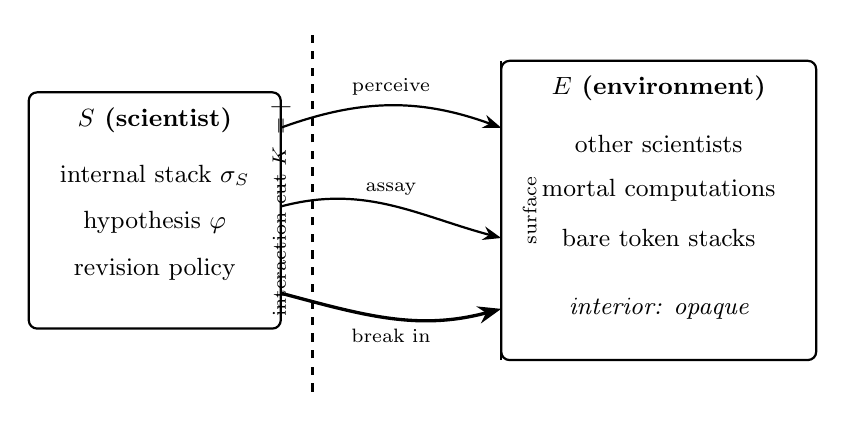
\begin{tikzpicture}[>=Stealth, font=\small]
  % scientist
  \draw[rounded corners=3pt, thick] (-4.6,-1.5) rectangle (-1.4,1.5);
  \node at (-3.0,1.15) {\bfseries $S$ (scientist)};
  \node at (-3.0,0.45) {internal stack $\sigma_S$};
  \node at (-3.0,-0.15) {hypothesis $\varphi$};
  \node at (-3.0,-0.75) {revision policy};
  % environment
  \draw[rounded corners=3pt, thick] (1.4,-1.9) rectangle (5.4,1.9);
  \node at (3.4,1.55) {\bfseries $E$ (environment)};
  \node at (3.4,0.85) {other scientists};
  \node at (3.4,0.25) {mortal computations};
  \node at (3.4,-0.35) {bare token stacks};
  \node at (3.4,-1.25) {\itshape interior: opaque};
  % the cut
  \draw[very thick, dashed] (-1.0,-2.3) -- (-1.0,2.3);
  \node[rotate=90, anchor=south] at (-1.15,0) {\scriptsize interaction cut $K \;=\; \mid$};
  % surface
  \draw[thick] (1.4,-1.9) -- (1.4,1.9);
  \node[rotate=90, anchor=north] at (1.55,0) {\scriptsize surface};
  % arrows
  \draw[->, thick] (-1.4,1.05) to[out=20,in=160] node[above,pos=.5]{\scriptsize perceive} (1.4,1.05);
  \draw[->, thick] (-1.4,0.05) to[out=15,in=165] node[above,pos=.5]{\scriptsize assay} (1.4,-0.35);
  \draw[->, very thick] (-1.4,-1.05) to[out=-15,in=195] node[below,pos=.5]{\scriptsize break in} (1.4,-1.25);
\end{tikzpicture}
\caption{The cut. Perception evaluates structural predicates at the surface; an assay reaches across
and perturbs; a break-in passes the surface and is fatal to what lies behind it. There is no fourth
route, and the three are ordered by both what they reveal and what they destroy
(\S\ref{sec:exposure}).}
\label{fig:cut}
\end{figure}

\section{The logic, and senses}
\label{sec:logic}

\subsection{What the generator supplies}

We recall only what we use, following \cite[\S2]{ClassifierNote}. The \rhoc\ calculus has term formers
$0$, $\ast n$, $n!(Q)$, $\texttt{for}(x \leftarrow n)P$, parallel composition, and $@P$; parallel
composition carries an associative--commutative equational theory and there is a single communication
rewrite. Feeding this presentation to the generator yields:

\paragraph{Structural connectives.} One connective per term former. We write $\mathrm{out}(n)\varphi$
for the predicate holding of $n!(Q)$ with $Q \models \varphi$, and $\mathrm{in}(n)\varphi$ for the
analogue on receipts. Because $\mid$ is associative--commutative, the generated connective for
parallel composition is a separating conjunction:
\[
P \models \varphi \mid \psi \iff P \equiv Q \mid R \text{ with } Q \models \varphi,\; R \models \psi .
\]

\paragraph{Behavioural modalities.} One primitive modality $\langle K_j \rangle$ per rewrite rule and
choice of redex position, labelled by the one-hole context in which the step fires.

\paragraph{Name predicates.} A name is a quoted process, so
\[
n \models @\varphi \iff n = @P \text{ with } P \models \varphi ,
\]
which is namespace logic \cite{NamespaceLogic}: one describes a namespace by a property rather than
enumerating it. \S\ref{sec:forced} shows this is not a convenience but a requirement.

\paragraph{Restriction, fixed point, grading.} The hidden-name quantifier
$P \models \mathsf{H}x.\varphi$ iff $P \equiv \texttt{new } x \texttt{ in } Q$ with
$Q \models \varphi$ and $x$ fresh; the greatest fixed point $\nu X.\varphi$ with $X$ positive; and
graded separation $\varphi \mid_k \psi$, which splits a term under $\mathsf{H}$ with exactly $k$
shared restricted names \cite[\S2.3]{ClassifierNote}.

\subsection{The structural predicates are admitted, and they are senses}

In \cite{ClassifierNote} the structural predicates are wielded by an analyst standing outside the
term, holding it in hand, free to count its gates and test its decompositions. That is not the
scientist's situation, and admitting the structural predicates without saying where they may be
applied would hand the scientist an oracle and destroy the isolation premise of \S\ref{sec:cut}.

The discipline that saves them is that a sense is a structural predicate evaluated \emph{at the
surface}.

\begin{definition}[Depth]
The \emph{depth} $d(\varphi)$ of a structural formula is the maximal nesting of term-former
connectives and prefixes occurring in it, with $d(\top) = 0$, $d(\mathrm{out}(n)\varphi) =
d(\mathrm{in}(n)\varphi) = 1 + d(\varphi)$, $d(\varphi \mid \psi) = \max(d(\varphi), d(\psi))$,
$d(\mathsf{H}x.\varphi) = 1 + d(\varphi)$, and $d(@\varphi) = d(\varphi)$.
\end{definition}

\begin{definition}[Sensing, and its price]
\label{def:sense}
For $W \equiv S \mid E$, the scientist $S$ may evaluate $\varphi$ against $E$ whenever
$d(\varphi) \le \alpha$, where $\alpha$ is $S$'s \emph{acuity}; the evaluation debits $S$'s stack by
$\kappa_{\mathrm{sense}}(d(\varphi))$, a monotone schedule. Acuity is not a fixed endowment: $\alpha$
is whatever $S$ can currently pay for.
\end{definition}

Two comments. First, the depth grading is what keeps perception from being an oracle: seeing deeper
costs more, so the interior of $E$ is not free, it is merely expensive, and past a point unaffordable.
Second, $d(@\varphi) = d(\varphi)$ rather than $1 + d(\varphi)$ is deliberate and records the third
grade of access: opening a name one holds is not a passage through a surface, because one already
holds it. Reflection is cheap for exactly the reason predation is not.

\begin{table}[t]
\centering
\begin{tabular}{@{}llll@{}}
\toprule
\textbf{grade} & \textbf{instrument} & \textbf{applies to} & \textbf{price} \\
\midrule
perception & $\mathrm{out}, \mathrm{in}, \mid, \mid_k, \mathsf{H}$ & the surface of $E$ &
$\kappa_{\mathrm{sense}}(d)$, monotone in depth \\
interaction & $\langle K \rangle \varphi$ & the behaviour of $E$ & one rendezvous per step, and time \\
reflection & $@\varphi$ & names $S$ holds & a computation on a name; no communication \\
\bottomrule
\end{tabular}
\caption{The three grades of access. The ladder is also an ordering by invasiveness
(\S\ref{sec:exposure}), and in the opposite direction.}
\label{tab:access}
\end{table}

\section{Hypotheses, assays, and the \texttt{where} clause}
\label{sec:assay}

\subsection{The embedding, in operational position}

An embedding of the logic into the calculus is what lets \rhoc\ computations compute over hypotheses.
The obvious construction --- reify formulae as data, write an interpreter --- works but is
unsatisfying, because the scientist must then carry the interpreter and the interpreter is not part of
the theory. The variant of \rhoc\ whose for-comprehension carries a \texttt{where} clause
\cite[\S9]{Omnibus} does better. Its general form is
\[
\texttt{for}\big( p_{11} \leftarrow c_{11} \,\&\, \cdots \,;\, \cdots \,;\, p_{1n} \leftarrow c_{1n}
\,\&\, \cdots \ \texttt{where}\ \vartheta \big) P
\]
with $\&$ joining within a group, $;$ separating groups, and $\vartheta$ a condition drawn from the
booleans over ground formulae, spatial connectives, and the context-labelled modality, in which the
variables bound by the preceding clauses may be mentioned. A guard is a formula in operational
position. Hence:

\begin{quote}
\itshape A hypothesis installed as a guard is an experiment, and a confirmation is a rendezvous.
\end{quote}

The checker is the reduction rule. Nothing is carried, nothing is interpreted, and the cost of testing
a hypothesis is metered by the same apparatus that meters everything else --- which is essential here,
since an unpriced hypothesis test would be an oracle and would collapse the entire motivational story
of \S\ref{sec:game}.

\subsection{The assay}

\begin{definition}[Assay]
\label{def:assay}
An \emph{assay} is a pair $(K, \varphi)$ of a probe context $K$ and a predicted property $\varphi$,
realised on a probe channel $p$ as
\begin{lstlisting}
   K[ ... ]                                        // the probe: perturb the environment
 | for (x <- p where phi(x)) { confirm!(*x) }       // prediction holds
 | for (x <- p where ~phi(x)) { refute!(*x) }       // prediction fails
\end{lstlisting}
\end{definition}

The negation in the second guard is what makes this more than an expression of hope. In a concurrent
setting a guard that simply fails to fire is indistinguishable from a guard still waiting, so a naive
encoding of falsification cannot tell refutation from patience. The complementary pair repairs this.

\begin{proposition}[Trichotomy]
\label{prop:trichotomy}
Let $A = (K,\varphi)$ be an assay on probe channel $p$, with $\varphi$ decidable on the received term
within the ambient budget. Then for each message arriving on $p$ exactly one of the two guards is
enabled, and the assay yields one of three outcomes: \textsc{confirm}, \textsc{refute}, or $\bot$,
where $\bot$ occurs exactly when no message arrives on $p$ before the budget for $A$ is exhausted.
\end{proposition}

\begin{proof}[Proof sketch]
$\varphi$ and $\lnot\varphi$ partition the terms on which both are decidable, so at most one guard is
enabled per message and the two receipts do not race. If a message arrives and the budget suffices to
decide $\varphi$ on it, one guard fires. Otherwise no output occurs on either \texttt{confirm} or
\texttt{refute}, which is the residual case.
\end{proof}

We stress that $\bot$ is not a defect. It is the honest residue: the environment did not answer, and
no amount of logical apparatus can distinguish that from an environment that would have answered
later. What it does is separate that genuine ignorance from falsity, which the naive encoding conflates.

\subsection{Refutation is budget-relative, and that fixes the fragment}

\begin{proposition}[Asymmetry of the modalities]
\label{prop:asymmetry}
Let $\varphi = \langle K \rangle \psi$. Then \textsc{confirm} is a finite witness for $\varphi$, while
no finite run witnesses $\lnot \varphi$. Dually for $\varphi = [K]\psi$: refutation is finite,
confirmation is not.
\end{proposition}

The consequence is the note's first structural fact about mortality. A scientist with a finite budget
can only run assays whose outcome is decided within that budget, so the fragment of the ideal logic it
can actually test is the one bounded in modal depth and fixed-point unfolding. That fragment is not
adequate --- a logic whose model checking terminates never is, for a Turing-complete host
\cite[\S1.3]{ClassifierNote}. Therefore:

\begin{quote}
\itshape A mortal scientist necessarily holds a non-adequate theory, and which non-adequate fragment
it holds is fixed by what it can pay for. The budget is the inductive bias.
\end{quote}

This is not a limitation we regret. It is the formal content of the observation that finite creatures
have finite theories, and it locates the inductive bias somewhere unusually concrete: not in a prior,
not in a regulariser, but in a token stack.

\section{The hypothesis space is the relaxation lattice}
\label{sec:lattice}

We do not need to invent a space of hypotheses. \cite[\S3.3]{ClassifierNote} constructs one and calls
it something else.

Recall the construction. For a process $P$, a \emph{characteristic formula} $\chi_P$ is satisfied by
exactly the processes equivalent to $P$; it turns an equivalence question into a model-checking
question. Beneath $\chi_P$ sits a lattice of progressively weaker formulae obtained by forgetting
parts of it --- the recursion, the continuations, a private name --- each forgetting yielding a
coarser predicate that more processes satisfy. In \cite{ClassifierNote} this lattice is where a
classifier's dials live. Here it is the space the scientist moves in.

\begin{definition}[Revision]
A \emph{revision} is a move on the relaxation lattice: \emph{generalisation} forgets a conjunct and
moves down, \emph{specialisation} restores one and moves up. A scientist's trajectory is a walk
$\varphi_0, \varphi_1, \varphi_2, \ldots$ on this lattice.
\end{definition}

\begin{definition}[Stratified distance]
For $\varphi, \psi$ agreeing on all approximants below stage $n$ and differing at $n$, set
$d(\varphi, \psi) = 2^{-n}$, where the stages are the $\nu$-unfolding approximants
$\nu^0 \supseteq \nu^1 \supseteq \cdots$. This is an ultrametric.
\end{definition}

The stratification is not chosen for convenience: it is how bisimulation is already approximated, it
grades with modal depth, and by Proposition~\ref{prop:asymmetry} modal depth is what the budget
bounds. Distance, depth, and cost are therefore one graded structure rather than three, which is the
main reason to prefer this metric to a measure-theoretic one on denotations.

\begin{proposition}[The limit of inquiry is unaffordable]
\label{prop:limit}
Let $E$ be an environment whose behaviour is not eventually structural in the sense of
\cite[Rem.~6]{ClassifierNote} --- that is, whose recursion follows the reduction rather than a finite
structural cycle. Then $\chi_E$ is not exact at any finite unfolding, and no scientist with a finite
token supply can install it as a guard.
\end{proposition}

So $\chi_E$ --- the complete theory of the environment --- sits at the top of the lattice as a limit
the scientist approaches and never reaches. Science converges \emph{along} the lattice.

\begin{remark}[When a finite theory is complete]
The converse case is worth naming because it is the good one. \cite[Rem.~6]{ClassifierNote} observes
that a recursion following the \emph{structure} rather than the reduction is exact at a finite
unfolding: for a diagram with $2n$ arcs, $\nu^{2n} = \nu$ on the nose. Read for the scientist, this
says that a finite theory is complete exactly when the environment's regularity is structural.
Recursions that follow the reduction are the unbounded ones. This is a serviceable formal criterion
for which subject matters admit closed sciences and which do not, and we suspect it is more useful
than it looks.
\end{remark}

\section{The game}
\label{sec:game}

\subsection{Conservation}

Tokens are conserved and never minted. Write $\Theta$ for the total supply of the world. The cost
monad's ledger law and the history monad's record together give, globally,
\[
\sigma + \kappa \;=\; \sigma_0 \;=\; \Theta ,
\]
where $\sigma$ is the total still held in live stacks and $\kappa$ the total spent. Spent tokens do
not vanish; they migrate into the record. So the free supply is monotonically non-increasing, the
accumulation of $\kappa$ is the arrow of time, and there is no primary producer. The whole game is a
finite race.

\begin{remark}[Science is entropy production]
The aggregate effect of every scientist in the world is to convert free tokens into history. This is
the precise form of the observation that the cost of remembering is the cost of doing science: the
record is made of spent tokens. It also means predation is not profit in any global sense --- it is
the purchase of someone else's remaining time.
\end{remark}

\subsection{Working in the image}
\label{sec:image}

Because \rhoc\ is Turing complete, cost-accounted \rhoc\ translates back into \rhoc: there is an
internalising encoding $\enc{-} : \Crho \to \rhoc$ that represents the located token stacks in the
undecorated calculus \cite[\S6]{Omnibus}. Without loss of generality we may therefore avail ourselves
of the cost-accounted syntax where that is convenient and of the channels at which token stacks are
located where that is convenient.

\begin{definition}[Metabolic channel]
\label{def:metabolic}
Under $\enc{-}$, a located stack becomes a message at a name. We call that name the \emph{metabolic
channel} $m_P$ of the computation $P$, and we call
\[
m_P!(\sigma) \;\mid\; \texttt{for}(t \leftarrow m_P)\{\, \text{debit};\ m_P!(\sigma')\ \mid\ \cdots \,\}
\]
the \emph{reclaim--debit--reissue} cycle. A mortal computation is a term equipped with a metabolic
channel executing this cycle, with a strictly positive burn rate.
\end{definition}

\begin{remark}[Metabolism is a race condition]
Living requires exposing one's stack as a message, if only for the instant between reclaiming and
reissuing. Computing is therefore racing others to one's own stack. We did not put this in; it is
what the comm rule does with Definition~\ref{def:metabolic}.
\end{remark}

\begin{definition}[Harvest, death]
\label{def:harvest}
A \emph{harvest} of $P$ by $S$ is the receipt $\texttt{for}(t \leftarrow m_P)$ performed by $S$. It is
an ordinary communication and requires no new rewrite rule. $P$ \emph{dies} when it cannot fund its
next step: the linear receipt consumed the message it was going to reclaim.
\end{definition}

So eating is a receive, death is starvation, and defence is restriction. All three are already in the
calculus.

\begin{remark}[One ledger]
The translation is not cost-free: simulating the metering costs \rhoc-steps. We therefore adopt one
metering convention throughout and state it once. \emph{Costs are always read in the decorated
calculus $\Crho$; the image is used only for the mechanics of transfer.} This matters because the
central inequalities of \S\ref{sec:exposure} and \S\ref{sec:distributions} are statements about ratios
of costs, and a non-uniform translation overhead would move their boundaries. It is the same
discipline of keeping levels distinct that governs running $\mathcal{C}$ on an
$\mathcal{H}$-equipped model.
\end{remark}

\subsection{Predation is the failure of internalisation to be faithful}

Here is the observation that we take to be the note's chief structural contribution.

In $\Crho$ a located stack is inviolable. That is not an accident of presentation; it is precisely
what the located-stack discipline and the ambient-authority fix were built to guarantee. No rewrite
takes your stack, because the stack is not the sort of thing a rewrite addresses.

In the image $\enc{\Crho} \subseteq \rhoc$ the stack is a message at a name, and any process holding
that name may receive it.

These are not the same situation, and the encoding is not faithful against arbitrary \rhoc\ contexts.
It is faithful against \emph{images of $\Crho$ contexts} --- which is exactly the refinement of
\cite{Probing}: an encoding may only be probed by the encodings of source contexts, since arbitrary
target contexts see strictly more and would never permit bisimulation preservation. Therefore:

\begin{theorem}[Predators are non-image contexts]
\label{thm:predator}
Let $\enc{-} : \Crho \to \rhoc$ be the internalising encoding and let $C[-]$ be a \rhoc\ context. If
$C$ lies in the image of $\enc{-}$ on contexts, then $C$ cannot harvest: the stack of any
$\enc{P}$ plugged into $C$ is preserved, since the source discipline forbids the corresponding step.
If $C$ lies outside the image and holds $m_P$, it may harvest. Hence the predatory contexts are
exactly the non-image contexts holding a metabolic name.
\end{theorem}

\begin{proof}[Proof sketch]
Faithfulness of $\enc{-}$ against image contexts is the hosting condition of \cite{Probing}: every
step available to $C[\enc{P}]$ with $C = \enc{C'}$ is the image of a step of $C'[P]$ in $\Crho$, and
no step of $\Crho$ removes a located stack from a term. A context outside the image is under no such
constraint; a bare receipt on $m_P$ is such a context and takes the stack.
\end{proof}

\begin{quote}
\itshape The decorated calculus is the world in which property rights hold. Its image is the state of
nature. The ecology lives in the gap, and eating is what the erasure theorem's side condition was
protecting against.
\end{quote}

This gives the game a rulebook rather than a stipulation.

\begin{definition}[The game]
\label{def:game}
A \emph{game} is a choice of admitted context class $\mathcal{A}$ with
$\enc{\Crho\text{-}\mathrm{Ctx}} \subseteq \mathcal{A} \subseteq \rhoc\text{-}\mathrm{Ctx}$.
\end{definition}

The two endpoints are degenerate: $\mathcal{A} = \enc{\Crho\text{-}\mathrm{Ctx}}$ is decorated
cost-accounted \rhoc\ with no game at all, and $\mathcal{A} = \rhoc\text{-}\mathrm{Ctx}$ is total war
in which any context may take anything it can address. The interesting point is the middle one:

\begin{definition}[Capability gating]
The \emph{capability-gated} game admits those contexts that \emph{derive} $m_P$ from structure they
can perceive, and excludes those that are simply handed it.
\end{definition}

Since names are unforgeable, derivation is real work, and it is the work namespace logic does:
describing a namespace by a property rather than enumerating it. Under capability gating, foraging is
name discovery and a hypothesis is a namespace description that either does or does not locate real
tokens. Everything below is stated for the capability-gated game.

\subsection{The foraging inequality}

Conservation has an immediate consequence which we will lean on repeatedly: harvest is not
automatically profitable, because finding and opening a stack costs tokens drawn from the same
conserved supply.

\begin{proposition}[Foraging inequality]
\label{prop:foraging}
A harvest of $P$ by $S$ credits $S$ on balance only if
\[
\sigma_P \;>\; \kappa_{\mathrm{sense}}(\delta_P) \;+\; \kappa_{\mathrm{assay}} \;+\;
\kappa_{\mathrm{break}},
\]
where $\sigma_P$ is the stack recovered and $\delta_P$ the depth at which $m_P$ lies concealed.
\end{proposition}

\begin{corollary}[The profitable band]
\label{cor:band}
Since a well-stocked computation can afford deeper concealment --- raising $\kappa_{\mathrm{sense}}$
--- while a poorly stocked one offers little $\sigma_P$, viable prey occupy a band: too poor is not
worth opening, too rich is not worth cracking.
\end{corollary}

This is optimal foraging theory, and we did not import it; it is what Proposition~\ref{prop:foraging}
says once concealment is priced by Definition~\ref{def:sense}. It is also the inequality whose sign
change draws the phase boundaries of \S\ref{sec:distributions}.

\section{Destructive assay forces a logic of namespaces}
\label{sec:forced}

Harvest ends the prey's computational life. That single decision has a consequence for the hypothesis
language which we did not expect and which we now regard as the best available answer to ``why
namespace logic.''

\begin{proposition}[One specimen, one measurement]
\label{prop:onespecimen}
Let $P$ be a mortal computation and let $S$ harvest it. Then no further assay may be run against $P$.
Consequently a hypothesis whose subject is the individual $P$ has zero expected yield after its own
first test.
\end{proposition}

\begin{proof}[Proof sketch]
By Definition~\ref{def:harvest} the harvest consumes $m_P$'s message and $P$ cannot fund a further
step, so $P$ contributes no further transitions and no further surface. A hypothesis $\varphi$ whose
denotation is $\{P\}$ is therefore, after the test, a predicate with empty extension among live
computations; whatever it cost to form and hold, it cannot be recouped.
\end{proof}

\begin{corollary}[Induction is forced]
\label{cor:induction}
In an ecology with destructive assay, the only hypotheses with positive expected yield are those whose
subject is a \emph{class} of computations. The hypothesis language must therefore be able to describe
a collection by a property rather than by enumeration.
\end{corollary}

That is namespace logic's definition. So the logic is not adopted for elegance or for uniformity with
a companion note; it is what survives the game. Induction --- the move from the specimen to the kind
--- is not an epistemic virtue the scientist is asked to display but the only strategy that pays when
each specimen affords exactly one measurement.

\begin{remark}[The biological reading]
Destructive assay is not exotic. Large parts of experimental biology sacrifice the animal, and the
inferential structure of those fields is exactly the one Corollary~\ref{cor:induction} describes:
because you cannot re-measure the individual, everything must be said about the strain, the cohort, or
the genotype. The formal setting reproduces the methodological consequence, which we take as evidence
that the modelling is not merely decorative.
\end{remark}

\section{Exposure, and the price of being known}
\label{sec:exposure}

\subsection{The exposure lemma}

The prey's optimal defence in a world of predators looks, at first, unbeatable. Restrict everything.
A fully closed computation is a live $\tau$-network with no free names; no context can communicate
with it; and by the pessimism of \cite[\S1]{ClassifierNote} its observable behaviour carries almost no
information. It cannot be perceived, so its metabolic channel cannot be derived, so it cannot be
harvested.

It also cannot eat.

\begin{lemma}[Exposure]
\label{lem:exposure}
Let $P$ be a mortal computation with strictly positive burn rate and no free names. Then $P$ performs
no harvest, its stack is monotonically decreasing, and $P$ dies in finitely many steps.
\end{lemma}

\begin{proof}[Proof sketch]
Harvest is a receipt on a metabolic name $m_Q$ belonging to some $Q$ outside $P$
(Definition~\ref{def:harvest}). If $\fn(P) = \emptyset$ then no such $m_Q$ occurs free in $P$, and
since restriction is not eliminated by reduction, none becomes free. So no receipt of $P$ can fire on
a name of another computation, and $P$'s stack receives no credits. With a positive burn rate it
therefore reaches zero in at most $\lceil \sigma_P / \varepsilon \rceil$ steps, where $\varepsilon$ is
the minimum debit.
\end{proof}

\begin{corollary}[Concealment is a luxury of the starving]
\label{cor:conceal}
Metabolic viability lower-bounds observability: any computation that survives indefinitely must expose
surface, hence must be perceivable, hence is in principle predictable and so in principle edible.
\end{corollary}

The predator's counter-move is now legible, and it is a reading of \cite[Rem.~2]{ClassifierNote}
turned around. Restriction makes a name unobservable but not undescribable; $\mathsf{H}x.\varphi$
reaches under the binder and speaks about what is hidden. A predator therefore attacks what it cannot
observe by \emph{describing} it, which is why the spatial layer and not the modal one is the hunting
instrument, and why senses had to be admitted in \S\ref{sec:logic} for the game to be non-trivial at
all.

\subsection{The invasiveness ladder}

Table~\ref{tab:access} ordered the three grades of access by what they reveal. They are ordered in the
opposite direction by what they destroy.

\begin{table}[h]
\centering
\begin{tabular}{@{}llll@{}}
\toprule
\textbf{engagement} & \textbf{effect on the subject} & \textbf{information} & \textbf{nutritive?} \\
\midrule
perceive & none & surface only & no \\
assay & perturbs; the environment changes & behaviour under one probe & no \\
break in & fatal & the whole interior, as structure & yes \\
\bottomrule
\end{tabular}
\caption{Information gain and subject survival are in strict opposition, and only the fatal end of the
ladder pays.}
\label{tab:ladder}
\end{table}

\begin{proposition}[The opposition is monotone]
Along the ladder, the information yielded is non-decreasing and the subject's residual life is
non-increasing; and the only rung that credits the scientist's stack is the last.
\end{proposition}

This is where the note's arc closes. A scientist that is very good at forming hypotheses locates
metabolic channels efficiently; locating them efficiently is eating efficiently; eating efficiently
exhausts the environment that was confirming the hypotheses. \emph{The better the theory, the faster
it destroys the conditions of its own confirmation.} Success is self-terminating, and no additional
assumption was needed to make it so.

\section{Mixed environments}
\label{sec:mixed}

The environment contains a mixture: bare token stacks, non-scientist mortal computations, and other
scientists. Each stratum behaves differently and the third is the interesting one.

\paragraph{Bare stacks} are the primary resource: inanimate, undefended, cheap to open, and finite.
They are what makes the shallow-and-external regime of \S\ref{sec:distributions} a regime in which
science does not pay --- when food lies in the open, senses suffice and a theory is pure overhead.

\paragraph{Non-scientist mortal computations} burn tokens and may have structure, but form no model.
They defend passively, by restriction, and are subject to Lemma~\ref{lem:exposure} like everyone else.

\paragraph{Scientists} model back, and three consequences follow.

\begin{proposition}[Scientists are preferred prey]
\label{prop:preferredprey}
Under equal stack size, a scientist exposes more surface than a passive mortal computation of the same
burn rate, since probing requires free names in addition to those needed for metabolism. By
Corollary~\ref{cor:conceal} it is therefore more readily perceived and its metabolic channel more
readily derived.
\end{proposition}

The most epistemically active agents are the most edible. We do not think this is an artefact.

\paragraph{Theory theft.} Reflection makes another scientist's hypothesis readable. A hypothesis in
guard position is a term; a term may be quoted; and $@\varphi$ inspects the quotation without
communicating. So a scientist may acquire a model by reading rather than by experimenting --- cheaper,
and not fatal to anyone. Whether honest science survives this depends on whether holding a model
requires exposing it, and in this calculus it does, because a guard is surface. We record the
equilibrium question as an open problem (\S\ref{sec:open}) rather than settle it.

\paragraph{Imagination.} Turing completeness plus reflection means a scientist may carry $\enc{-}$
itself as data and \emph{run} a model of a prey's metabolism inside its own budget, paying tokens to
avoid paying tokens.

\begin{proposition}[When imagination pays]
\label{prop:imagination}
Simulating a hunt is viable exactly when the cost of the simulation is below the expected cost of the
errors it prevents:
\[
\kappa_{\mathrm{sim}} \;<\; \Pr[\text{failed hunt}] \cdot \big(\kappa_{\mathrm{sense}} +
\kappa_{\mathrm{assay}} + \kappa_{\mathrm{break}}\big).
\]
\end{proposition}

This is the point at which the scientist stops being a reactive forager and becomes a planner, and it
is where the stacking of the cost and history monads acquires an interpretation that is not merely
formal: the simulated prey is itself a mortal computation, metered inside the predator's budget.

\section{Distributions over ecologies}
\label{sec:distributions}

\subsection{A world is a partition of a conserved quantity}

Because $\Theta$ is fixed and never minted, a world is a partition of $\Theta$ across loci together
with a structural assignment saying which loci are scientists, which are non-scientist mortal
computations, and which are bare stacks. The configuration space is graded by $\Theta$, and a
distribution over it is a microcanonical ensemble in the strict sense --- fixed total, distribution
over microstates. The analogy is exact rather than suggestive, and it is exact because conservation
is exact.

\begin{definition}[Configuration, ecology]
A \emph{configuration} is a finite multiset of mortal computations and bare stacks together with an
assignment of stack sizes summing to $\Theta$ and a designation of which computations carry a revision
policy. An \emph{ecology} is a configuration together with a distribution over the configurations
reachable from it.
\end{definition}

\subsection{Two order parameters, and a phase}

Two quantities govern the qualitative behaviour and they are independent:
\begin{itemize}
\item $\iota \in [0,1]$, the fraction of $\Theta$ already \emph{internal} to scientists rather than
loose in the environment;
\item $\delta \ge 0$, the mean \emph{concealment depth} of external stacks --- how far under
restriction and structure they lie, which by Definition~\ref{def:sense} sets the sensing cost of
finding them.
\end{itemize}

\begin{figure}[t]
\centering
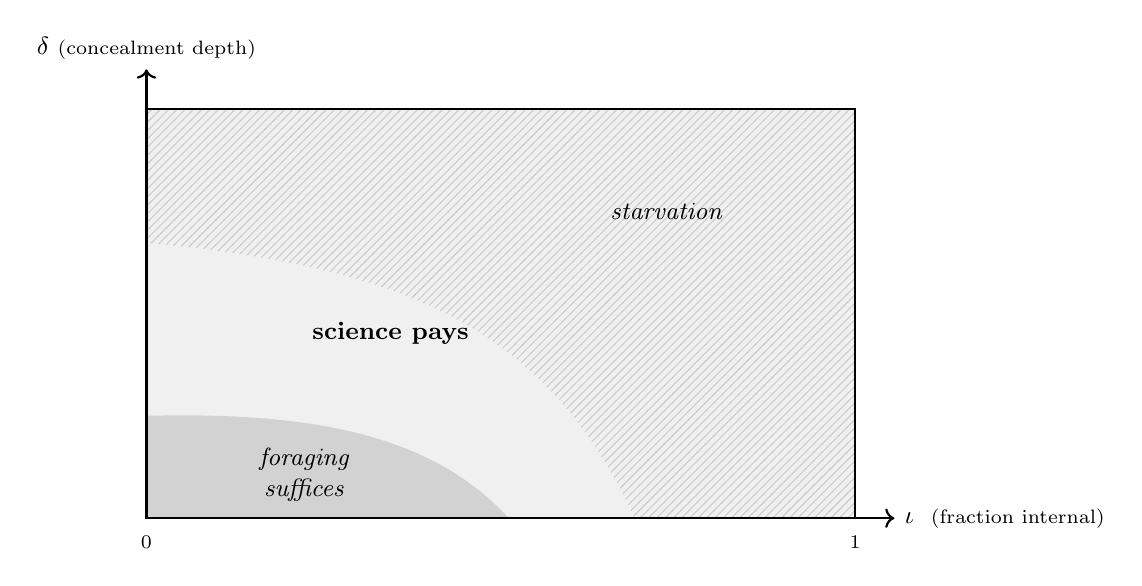
\begin{tikzpicture}[font=\small, scale=1.0]
  \fill[gray!12] (0,0) rectangle (9,5.2);
  % starvation region (high delta / high iota)
  \fill[pattern=north east lines, pattern color=gray!60, opacity=.55]
    (0,3.5) .. controls (3,3.2) and (5,2.6) .. (6.2,0) -- (9,0) -- (9,5.2) -- (0,5.2) -- cycle;
  % trivial foraging region (low delta)
  \fill[gray!35] (0,0) -- (0,1.3) .. controls (2,1.35) and (3.6,1.1) .. (4.6,0) -- cycle;
  \draw[thick] (0,0) rectangle (9,5.2);
  \node[align=center] at (2.0,0.55) {\itshape foraging\\ \itshape suffices};
  \node[align=center] at (3.1,2.35) {\bfseries science pays};
  \node[align=center] at (6.6,3.9) {\itshape starvation};
  \draw[->,thick] (0,0) -- (9.5,0) node[right] {$\iota$ \ \scriptsize(fraction internal)};
  \draw[->,thick] (0,0) -- (0,5.7) node[above, align=center] {$\delta$\ \scriptsize(concealment depth)};
  \node[below] at (0,-0.1) {\scriptsize $0$};
  \node[below] at (9,-0.1) {\scriptsize $1$};
\end{tikzpicture}
\caption{The phase diagram. When food lies shallow and in the open (low $\delta$), senses alone
suffice and a theory is overhead: the pure forager beats the scientist. When too much of $\Theta$ is
already internal, or lies too deep to be found for what it yields, discovery costs more than it
returns and everything starves. Hypothesis formation pays in the intervening band. Science is a phase,
not a universal advantage.}
\label{fig:phase}
\end{figure}

\begin{quote}
\itshape Science only pays in an intermediate band --- where food is neither free nor absent.
\end{quote}

We regard this as the most substantive empirical claim the construction makes, and it is a claim the
construction makes rather than one we impose: the boundaries of Figure~\ref{fig:phase} are where the
foraging inequality of Proposition~\ref{prop:foraging} changes sign. The low-$\delta$ boundary is
where $\kappa_{\mathrm{sense}}$ falls below the cost of holding a theory at all; the upper boundary is
where Proposition~\ref{prop:foraging} fails for every available $P$.

\subsection{Sampling}

The machinery for turning a configuration into a distribution and sampling trajectories through it is
not new work. The construction of \cite{StochSim} takes a decorated continued interactive GSLT, an
adequate spatial--behavioural logic, and a weight-map decoration to a Gillespie-style simulator,
framed as a functor from a Grothendieck construction of decorations into weighted coalgebras. That is
precisely what an ecology is: the weight map turns a configuration into a distribution, and the
Gillespie construction samples it. \S\ref{sec:functor} takes up what that fibred structure means here.

\section{The audit: what the assumptions already fix}
\label{sec:audit}

It is easy to build a machine that fits a story. We therefore separate, explicitly, what follows from
the commitments and what we chose.

\subsection{Forced}

\begin{table}[h]
\centering
\begin{tabular}{@{}p{0.42\textwidth}p{0.5\textwidth}@{}}
\toprule
\textbf{feature} & \textbf{forced by} \\
\midrule
the hypothesis language & OSLF applied to the \rhoc\ presentation; not designed \\
formulae denote bisimulation classes & adequacy of the generated logic \\
exactly three grades of access & the calculus offers no fourth (\S\ref{sec:cut}) \\
senses are structural predicates & admitting the structural layer, priced by depth \\
an assay is a guarded receipt & the \texttt{where} clause \\
refutation is budget-relative & Proposition~\ref{prop:asymmetry} \\
the hypothesis space & the relaxation lattice of \cite{ClassifierNote} \\
hypotheses must be about namespaces & destructive assay (Corollary~\ref{cor:induction}) \\
eating is an ordinary receipt & internalisation plus Turing completeness \\
death is failure to fund the next step & the cost monad \\
$\sigma + \kappa = \sigma_0$ globally & the history monad plus no minting \\
predators are non-image contexts & Theorem~\ref{thm:predator} \\
the exposure lemma & Lemma~\ref{lem:exposure} \\
optimal foraging, and its profitable band & conservation plus depth pricing
(Prop.~\ref{prop:foraging}) \\
information opposes survival & Table~\ref{tab:ladder} \\
\bottomrule
\end{tabular}
\end{table}

\subsection{Chosen}

\begin{table}[h]
\centering
\begin{tabular}{@{}p{0.42\textwidth}p{0.5\textwidth}@{}}
\toprule
\textbf{parameter} & \textbf{status} \\
\midrule
$\Theta$, the conserved total & free; sets the scale of the whole game \\
the initial configuration and its distribution & free; \S\ref{sec:distributions} \\
the admitted context class $\mathcal{A}$ & free; Definition~\ref{def:game}, and it is the rulebook \\
the pricing schedule $\kappa_{\mathrm{sense}}$, per-rewrite debits & free; the weight map \\
concealment depth $\delta$ of stacks & free; an order parameter \\
harvest all-or-nothing versus partial & free; we take all-or-nothing \\
the revision policy & free; this is the agent design, and we leave it open \\
\bottomrule
\end{tabular}
\end{table}

\begin{quote}
\itshape The physics is forced. The ecology and the psychology are the free parameters.
\end{quote}

Everything metabolic and everything epistemic follows from cost-accounted \rhoc\ together with the
logic it generates. What remains to be chosen is the weight map, the initial distribution, and how the
scientist thinks. We regard the smallness of that list as the principal evidence that the modelling
choices were not tuned to the conclusions.

\section{Is the assignment functorial?}
\label{sec:functor}

It is natural to ask whether ecologies are a functor of the theory: is there a functor from the
subcategory of cost-accounted graph-structured lambda theories to distributions over computational
ecologies of the kind described above? The answer is instructive, and it is no in a way that tells us
what the right question was.

\subsection{Not from the base}

Write $\CGSLT$ for the subcategory of cost-accounted GSLTs. The assignment
$\mathcal{C}(G) \mapsto$ ``its ecologies'' is not determined by $\mathcal{C}(G)$. Two different weight
maps --- two different pricing schedules on the same cost-accounted theory --- give different sensing
costs, hence different foraging inequalities, hence different phase boundaries in
Figure~\ref{fig:phase} and different distributions over trajectories. The object does not determine
the image.

\begin{proposition}[A fibration, not a functor]
\label{prop:fibration}
The ecologies form a fibration $\pi : \Eco \to \CGSLT$ whose fibre over $\mathcal{C}(G)$ is the class
of ecologies presentable in $\mathcal{C}(G)$, indexed by the decorations $\Dec(G)$. The assignment of
distributions is a functor out of the total space --- equivalently, out of the Grothendieck
construction $\textstyle\int_{\CGSLT} \Dec$ --- and not out of the base.
\end{proposition}

This is \cite{StochSim}'s theorem with a different label on the target: that construction already goes
from a Grothendieck construction of decorations into weighted coalgebras, and an ecology-with-a-
distribution is a weighted coalgebra.

\subsection{A canonical section}

There is nevertheless a rescue, and its shape is the interesting part.

\begin{proposition}[Cost is already a weighting]
\label{prop:section}
A cost-accounted GSLT is not decoration-free: the cost function is itself a weight map. Taking costs
as the weights selects a distinguished decoration for every object of $\CGSLT$, hence a section
$s : \CGSLT \to \Eco$ of $\pi$, and hence a genuine assignment of ecologies to objects.
\end{proposition}

So the honest statement is not ``there is a functor'' but ``there is a canonical one, and its
canonicity is exactly the observation that cost is already a weighting.'' Any other ecology over the
same theory is a re-weighting, and the deviation from the canonical section measures how far the
modeller's pricing departs from the theory's own.

\subsection{The morphisms must be logic-preserving}

Functoriality on morphisms is where a real correction is needed, and we think it is the most useful
thing this section contains.

The morphisms of $\GSLT$ are bisimulation-preserving maps, where the bisimulation is the
context-labelled one and is a congruence \cite{Omnibus}. But an ecology depends on \emph{spatial}
structure: concealment depth, which computations sit inside which, how a network separates when a
locus is removed. And the spatial layer strictly refines bisimulation --- this is the entire thesis of
\cite{ClassifierNote}, that separation says things no modal logic can say. So a bisimulation-preserving
map may scramble the spatial layer, changing sensing costs and foraging inequalities while preserving
behaviour exactly.

\begin{proposition}[Refinement of the morphism class]
\label{prop:morphisms}
The assignment of Proposition~\ref{prop:section} is not functorial on $\GSLT$-morphisms. It requires
morphisms preserving the \emph{generated logic} --- both the behavioural and the structural layers ---
which is a strictly narrower class, strictly because the structural layer strictly refines
context-labelled bisimulation.
\end{proposition}

The narrowing is not ad hoc. It is forced by the fact that the senses are structural: a morphism that
does not preserve what the senses see does not preserve the ecology, because it does not preserve what
it costs to find food.

\begin{conjecture}[Laxity]
\label{conj:lax}
Even over logic-preserving morphisms the induced map on distributions is only lax. An encoding may add
rewrite steps and so inflate costs, so the pushforward distorts; the natural target is distributions
ordered by stochastic dominance rather than distributions on the nose.
\end{conjecture}

We state this and do not chase it. The three-line summary for the reader in a hurry is: a fibration, a
canonical section via cost-as-weight, and a refinement of the morphism class forced by the senses being
structural.

\section{Proximate and ultimate scores}
\label{sec:scores}

The original motivation for this construction measured the delta between hypothesis revisions and
punished degradation. The game supersedes that mechanism as the \emph{ultimate} criterion --- survival
is the score, and it needs no adjudicator, no referee holding a mint, and no exogenous reward signal.
Two things fall out that we would otherwise have had to impose.

\begin{itemize}
\item \textbf{Vacuity is punished by hunger, not by rule.} The hypothesis $\top$ predicts nothing,
locates no metabolic channel, yields nothing, and starves. No informativeness term is needed in any
score function, because there is no score function.
\item \textbf{Occam's razor is metabolic.} A hypothesis is worth holding exactly when expected yield
exceeds $\kappa_{\mathrm{sense}} + \kappa_{\mathrm{assay}} + \kappa_{\mathrm{break}}$ plus the cost of
holding the formula itself. Description length and food are denominated in the same currency, so
minimum description length is derived rather than stipulated.
\end{itemize}

The revision delta nevertheless survives, demoted and better placed. A scientist cannot wait until it
dies to learn which way to walk the relaxation lattice, so it needs a local signal, and
$d(\varphi_n, \varphi_{n+1})$ together with the confirm/refute counts of \S\ref{sec:assay} is exactly
one. This is the proximate/ultimate distinction of behavioural ecology: viability is the ultimate
criterion, the revision delta is the proximate mechanism that tracks it, and neither is redundant.

\begin{remark}[The pragmatist's objection, and surplus]
It should be conceded plainly that this scientist is not a disinterested seeker of truth. Its
epistemology is metabolic, and truths that do not pay go unfunded. That is the standard objection to
pragmatism and we do not think it can be argued away. The construction does, however, have an unusually
concrete answer: \emph{surplus}. A scientist holding a stack larger than its foraging horizon requires
can afford inquiry that does not pay, and what it buys with the excess is curiosity. Basic research is
a metabolic luxury, available exactly to the well-fed, and in a world of conserved tokens it is
therefore rare and worth protecting. We note this and leave the moral to others.
\end{remark}

\section{Open problems}
\label{sec:open}

\begin{enumerate}
\item \textbf{Reproduction and regeneration.} Harvest here ends a computational life and nothing is
born, so every ecology runs down. Regeneration as reproduction is the companion note, and it is what
turns Figure~\ref{fig:phase} from a snapshot into a dynamics with a carrying capacity.

\item \textbf{The plagiarism equilibrium.} Reading a rival's model is cheaper than experimenting and
kills nobody, but holding a model requires exposing it as a guard. Under what pricing does honest
science survive theory theft, and is there a mixed equilibrium?

\item \textbf{Co-learning and non-stationarity.} When the environment is mostly scientists, the target
of every hypothesis is itself revising. Convergence becomes a fixed-point question rather than a
learning-theoretic one, and this is where we expect the geometry/matter corecursion to be readable as
learning.

\item \textbf{Laxity.} Conjecture~\ref{conj:lax}: is the induced map on distributions lax, and is
stochastic dominance the right order on the target?

\item \textbf{The revision policy.} We left the agent design open on purpose. Is there a policy on the
relaxation lattice that is optimal in the ecological sense --- maximising expected residual life
rather than predictive accuracy --- and does it look anything like the policies learning theory
recommends?

\item \textbf{Sharpening the phase boundary.} Figure~\ref{fig:phase} is drawn from the sign of a cost
inequality. Making its boundaries quantitative for a specific pricing schedule, via the sampling
construction of \cite{StochSim}, is the first computation to do.
\end{enumerate}

\begin{thebibliography}{99}

\bibitem{KnotsNote} L.\ G.\ Meredith. \emph{Knots as cost-accounted rholang processes: a
Dowker--Thistlethwaite-driven encoding and weak-bisimulation invariance.} F1R3FLY.io, 2026.

\bibitem{ClassifierNote} L.\ G.\ Meredith. \emph{Classifying knot diagrams with a spatial--behavioural
logic: a logic obtained for free from the encoding of knots as processes.} F1R3FLY.io, 2026.

\bibitem{Omnibus} \emph{Graph-structured lambda theories: a reference for the working developer.}
F1R3FLY.io, 2026.

\bibitem{Probing} L.\ G.\ Meredith. \emph{Probing universality: context-labelled bisimulation and a
relative refinement of Turing completeness for interactive GSLTs.} F1R3FLY.io, 2026.

\bibitem{CostMonad} L.\ G.\ Meredith. \emph{Cost accounting as a monad for continued graph-structured
lambda theories.} F1R3FLY.io, 2026.

\bibitem{History} L.\ G.\ Meredith. \emph{History as an endofunctor.} F1R3FLY.io, 2026.

\bibitem{StochSim} L.\ G.\ Meredith. \emph{Stochastic simulation for decorated ciGSLTs.} F1R3FLY.io,
2026.

\bibitem{Zeus} L.\ G.\ Meredith. \emph{Splitting the mind of Zeus: realizability, collection monads,
and the choice content of the McBride derivative in a finite-limits metalanguage.} F1R3FLY.io, 2026.

\bibitem{NamespaceLogic} L.\ G.\ Meredith and M.\ Radestock. Namespace logic: a logic for a reflective
higher-order calculus. In \emph{Trustworthy Global Computing}, LNCS 3705, Springer, 2005.

\bibitem{RHO} L.\ G.\ Meredith and M.\ Radestock. A reflective higher-order calculus. \emph{Electronic
Notes in Theoretical Computer Science} 141(5):49--67, 2005.

\bibitem{OSLF} \emph{Operational semantics in logical form (OSLF): a family of algorithms
auto-generating logics and type systems from graph-structured lambda theories.}

\bibitem{Caires} L.\ Caires. Behavioral and spatial observations in a logic for the pi-calculus. In
\emph{Foundations of Software Science and Computation Structures (FoSSaCS)}, LNCS 2987, Springer, 2004.

\bibitem{CairesCardelli} L.\ Caires and L.\ Cardelli. A spatial logic for concurrency (part I).
\emph{Information and Computation} 186(2):194--235, 2003.

\bibitem{Milner} R.\ Milner. Functions as processes. \emph{Mathematical Structures in Computer
Science} 2(2):119--141, 1992.

\bibitem{Plotkin} G.\ D.\ Plotkin. A structural approach to operational semantics. \emph{Journal of
Logic and Algebraic Programming} 60--61:17--139, 2004.

\bibitem{Landauer} R.\ Landauer. Irreversibility and heat generation in the computing process.
\emph{IBM Journal of Research and Development} 5(3):183--191, 1961.

\bibitem{Hinton} G.\ Hinton. The forward-forward algorithm: some preliminary investigations, 2022.
(Mortal computation.)

\bibitem{Gillespie} D.\ T.\ Gillespie. Exact stochastic simulation of coupled chemical reactions.
\emph{Journal of Physical Chemistry} 81(25):2340--2361, 1977.

\end{thebibliography}

\end{document}
